\documentclass[aspectratio=169]{beamer}
\usetheme{Madrid}
\usecolortheme{seahorse}
\usepackage[utf8]{inputenc}
\usepackage{amsmath,amssymb}
\usepackage{graphicx}
\usepackage{booktabs}
\graphicspath{{../../figures/}{../../figures/modeling/}}

\title[Predicción de resultados de fútbol]{Clasificación Multiclase de Resultados de Fútbol
a Escala Multi-Liga con Validación Temporal y Análisis de Significancia Estadística}
\subtitle{Minería de Datos (CC442) --- 2026-I}
\author[Pérez, Trujillo, Pezo]{Arbués Pérez Villegas \and Luis Trujillo Serva \and Sergio Pezo Jimenez}
\institute[UNI]{Universidad Nacional de Ingeniería --- Ciencia de la Computación}
\date{Julio 2026}

\begin{document}

% 1 -----------------------------------------------------------------
\begin{frame}[plain]
  \titlepage
\end{frame}

% 2 -----------------------------------------------------------------
\begin{frame}{Agenda}
  \begin{columns}[t]
    \column{0.5\textwidth}
    \textbf{Arbués --- Datos}
    \begin{enumerate}
      \item Motivación y problema
      \item Objetivos
      \item Dataset y EDA
      \item Preprocesamiento
    \end{enumerate}
    \textbf{Sergio --- Metodología}
    \begin{enumerate}\setcounter{enumi}{4}
      \item Arquitectura y validación
      \item Modelos y fundamentos
    \end{enumerate}
    \column{0.5\textwidth}
    \textbf{Luis --- Validación}
    \begin{enumerate}\setcounter{enumi}{6}
      \item Resultados y métricas
      \item Significancia (Wilcoxon)
      \item Interpretabilidad (SHAP)
      \item Discusión y conclusiones
    \end{enumerate}
  \end{columns}
\end{frame}

% 3 -----------------------------------------------------------------
\begin{frame}{Motivación y contexto}
  \begin{itemize}
    \item Predecir \textbf{local / empate / visitante} es un problema clásico de analítica deportiva.
    \item Difícil por dos razones:
    \begin{itemize}
      \item marcador bajo $\Rightarrow$ el \textbf{azar} pesa mucho;
      \item el \textbf{empate} es clase minoritaria y esquiva.
    \end{itemize}
    \item Pregunta de investigación: \emph{¿cuánto se puede predecir de forma honesta,
    sin usar las cuotas del mercado?}
  \end{itemize}
\end{frame}

% 4 -----------------------------------------------------------------
\begin{frame}{Definición formal del problema}
  Clasificación supervisada multiclase:
  \[
    g:\mathbb{R}^{d}\rightarrow\{H,\,D,\,A\}
  \]
  \begin{itemize}
    \item $\mathbf{x}\in\mathbb{R}^{d}$: características \textbf{previas} al partido.
    \item $H$ local, $D$ empate, $A$ visitante.
    \item Restricción \textbf{temporal}: nada de lo ocurrido durante/después del partido entra en $\mathbf{x}$.
  \end{itemize}
\end{frame}

% 5 -----------------------------------------------------------------
\begin{frame}{Objetivos}
  \begin{block}{General}
    Diseñar un pipeline reproducible y \textbf{sin fuga de datos} que compare nueve familias
    de modelos.
  \end{block}
  \begin{block}{Específicos}
    \begin{itemize}
      \item Líneas base (Dummy, Naive Bayes).
      \item Modelos del curso con fundamentación matemática.
      \item Gradient boosting moderno + ensamble.
      \item Métricas por clase y prueba de significancia.
    \end{itemize}
  \end{block}
\end{frame}

% 6 -----------------------------------------------------------------
\begin{frame}{Descripción del dataset}
  \textbf{Club Football Match Data (2000--2025)}
  \begin{itemize}
    \item $N = 230\,554$ partidos, múltiples ligas internacionales.
    \item Objetivo: \texttt{FTResult} $\in \{H, D, A\}$.
    \item Información pre-partido: Elo, forma, goles, historial. \textbf{Sin cuotas}.
    \item Escala superior a la literatura habitual (una liga, pocos miles).
  \end{itemize}
\end{frame}

% 7 -----------------------------------------------------------------
\begin{frame}{EDA I --- Desbalance de clases}
  \begin{columns}
    \column{0.52\textwidth}
    \begin{itemize}
      \item $H$ 44,6\% \; $A$ 28,9\% \; $D$ 26,5\%
      \item Razón de desbalance $= 1{,}68$.
      \item \alert{Consecuencia:} optimizar \emph{accuracy} premiaría al que siempre dice ``local''.
      \item $\Rightarrow$ optimizamos \textbf{F1 macro}.
    \end{itemize}
    \column{0.48\textwidth}
    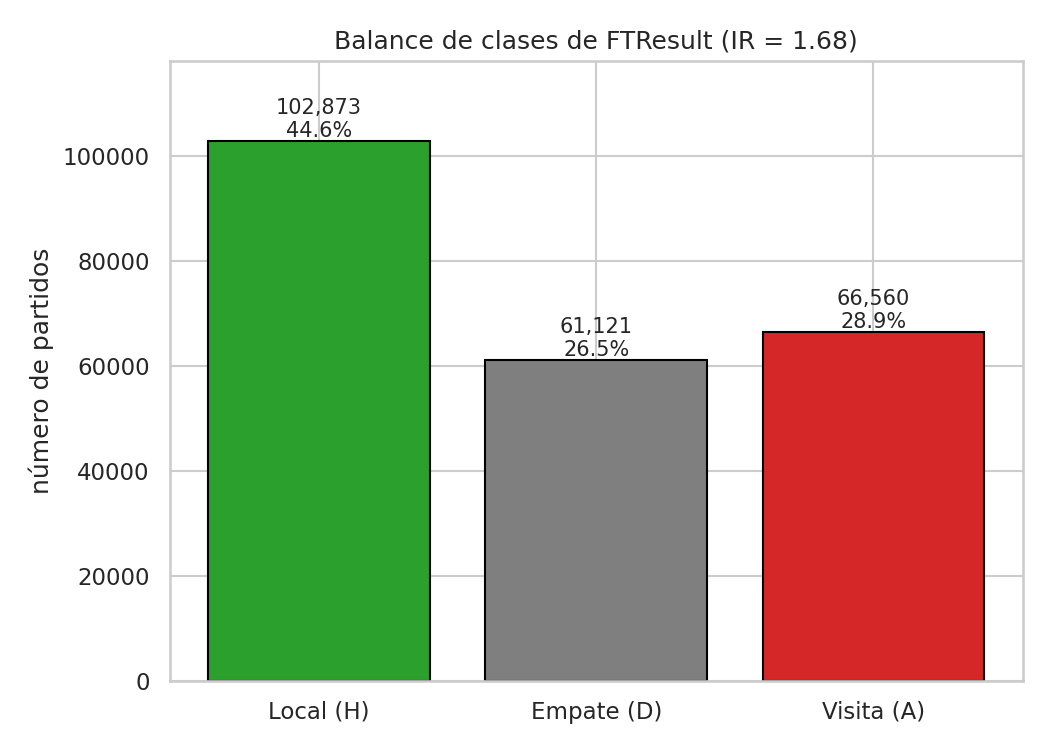
\includegraphics[width=\linewidth]{class_balance.png}
  \end{columns}
\end{frame}

% 8 -----------------------------------------------------------------
\begin{frame}{EDA II --- Elo y multicolinealidad}
  \begin{columns}
    \column{0.5\textwidth}
    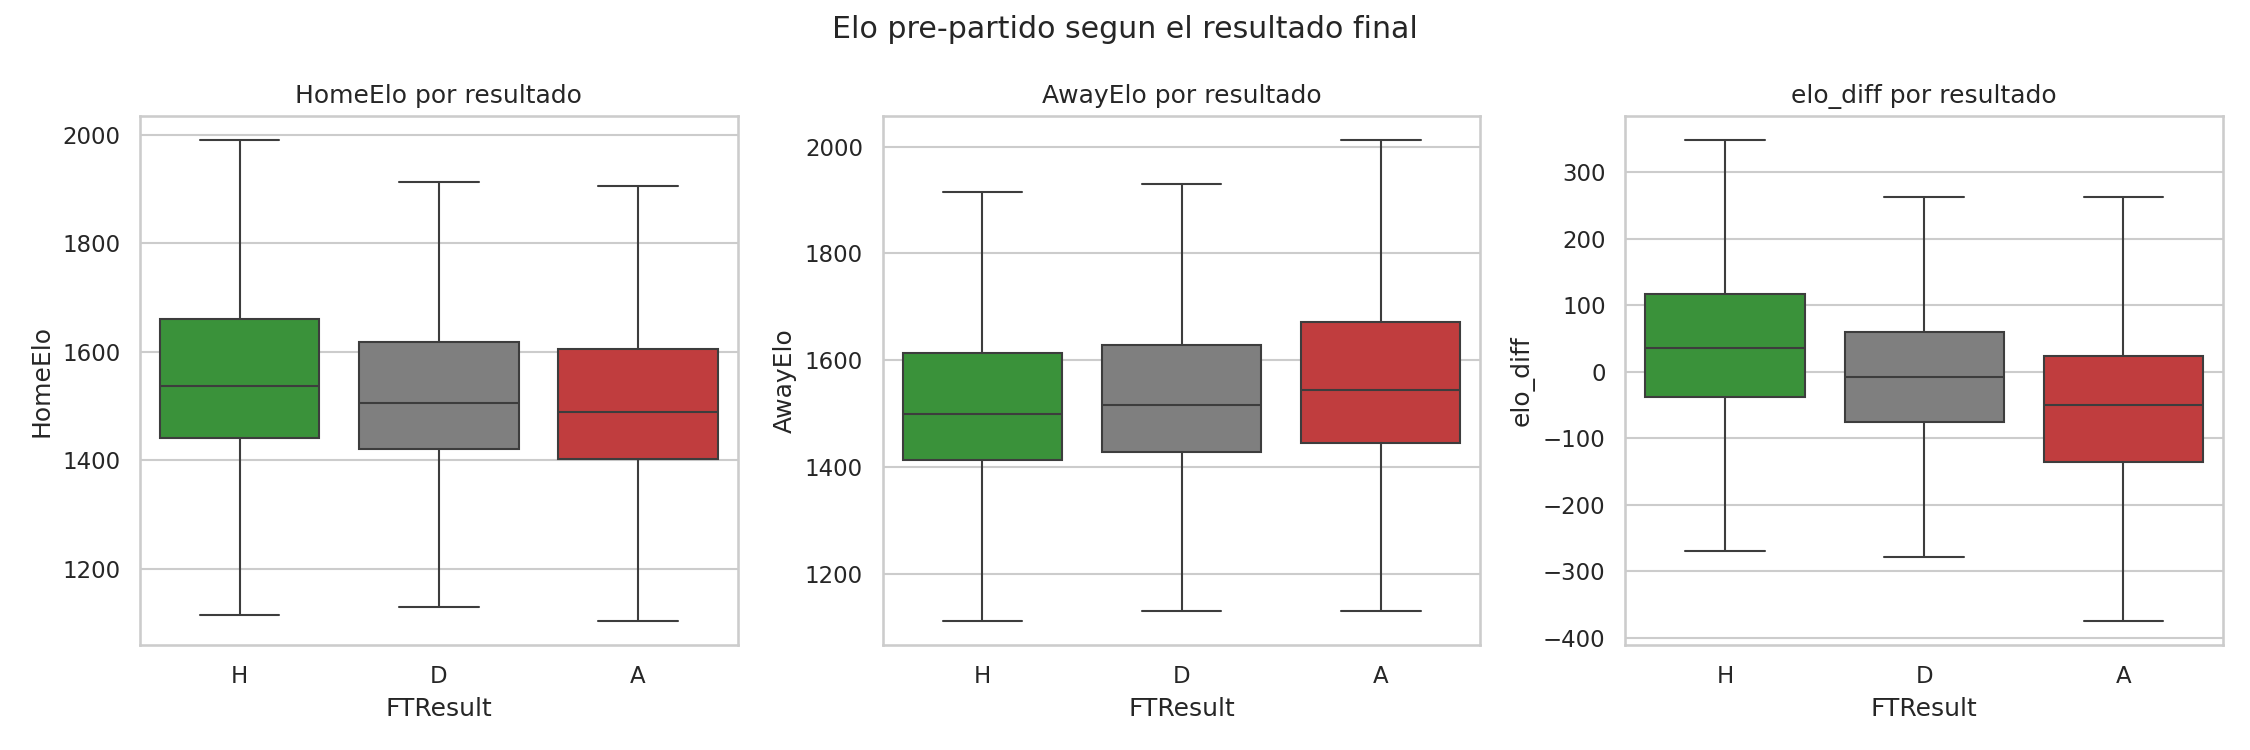
\includegraphics[width=\linewidth]{elo_by_result.png}
    \column{0.5\textwidth}
    \begin{itemize}
      \item La \textbf{diferencia de Elo} separa H$>$D$>$A, pero el empate queda \emph{en el medio}.
      \item $\Rightarrow$ frontera \textbf{no lineal} (favorece árboles/kernels).
      \item Multicolinealidad exacta (VIF $\to\infty$; 5 autovalores nulos).
      \item Elo ausente estructuralmente + deriva temporal (COVID).
    \end{itemize}
  \end{columns}
\end{frame}

% 9 -----------------------------------------------------------------
\begin{frame}{Pipeline de preprocesamiento}
  \begin{center}
  \footnotesize
  Datos crudos $\rightarrow$ limpieza anti-fuga $\rightarrow$ reconstrucción de Elo
  $\rightarrow$ ingeniería de \emph{features} $\rightarrow$ \textbf{partición temporal}
  $\rightarrow$ estandarización (\emph{fit} en train) $\rightarrow$ modelado
  \end{center}
  \vspace{1em}
  \begin{itemize}
    \item Se descartan columnas post-partido (fuga) y cuotas (versión honesta).
    \item Estandarización y encoders ajustados \textbf{solo en entrenamiento}.
  \end{itemize}
\end{frame}

% 10 ----------------------------------------------------------------
\begin{frame}{Limpieza e imputación}
  \begin{itemize}
    \item \textbf{Elo faltante} ($\sim$35\%): NO imputar con 0.
    \begin{itemize}
      \item Reconstrucción por unión temporal ($\text{fecha}\le\text{fecha del partido}$).
      \item Ausencia estructural $\rightarrow$ bandera \texttt{elo\_missing}.
    \end{itemize}
    \item Forma y goles: imputación por mediana de entrenamiento.
    \item Estandarización Z-score con parámetros del train:
    \[ x'_{ij}=\frac{x_{ij}-\mu_{j,\text{train}}}{\sigma_{j,\text{train}}} \]
  \end{itemize}
\end{frame}

% 11 ----------------------------------------------------------------
\begin{frame}{Ingeniería de características y partición}
  \begin{columns}[t]
    \column{0.55\textwidth}
    \textbf{62 características} (solo pasado):
    \begin{itemize}
      \item diferencias de Elo, forma, goles;
      \item historial directo, descanso, rachas;
      \item banderas + one-hot de liga.
    \end{itemize}
    \column{0.45\textwidth}
    \textbf{Partición temporal}
    \begin{itemize}
      \item train $\le 2021$ (191k)
      \item val 2022--2023 (25k)
      \item test 2024--2025 (15k)
    \end{itemize}
    \alert{K-fold aleatorio = fuga.}
  \end{columns}
\end{frame}

% 12 ----------------------------------------------------------------
\begin{frame}{Arquitectura de la metodología}
  \begin{itemize}
    \item Hiperparámetros: \texttt{TimeSeriesSplit} (5) \textbf{dentro} de train.
    \item Selección entre familias: conjunto de \textbf{validación} (2022--2023).
    \item Reporte final: conjunto de \textbf{prueba} (2024--2025), intacto.
    \item Métrica optimizada: \textbf{F1 macro}
    \[ \mathrm{F1}_{\text{macro}}=\tfrac{1}{3}\sum_{c\in\{H,D,A\}}\frac{2P_cR_c}{P_c+R_c} \]
  \end{itemize}
\end{frame}

% 13 ----------------------------------------------------------------
\begin{frame}{Modelo A --- lineales y de margen}
  \begin{itemize}
    \item \textbf{Regresión logística} (softmax + L2 = Tikhonov):
    \[ \mathcal{L}=-\sum_i\log P(y_i\mid x_i)+\lambda\lVert W\rVert^2 \]
    la L2 vuelve invertible la matriz singular por colinealidad.
    \item \textbf{SVM}: maximiza el margen $1/\lVert w\rVert$; \emph{kernel} RBF
    $K(x,x')=\exp(-\gamma\lVert x-x'\rVert^2)$ $\Rightarrow$ frontera no lineal.
    \item \textbf{Árbol}: maximiza la ganancia de información $IG=H(Y)-H(Y\mid X)$.
  \end{itemize}
\end{frame}

% 14 ----------------------------------------------------------------
\begin{frame}{Modelo B --- ensambles y boosting}
  \begin{itemize}
    \item \textbf{Random Forest}: bagging; al restringir a $m<p$ atributos
    \textbf{descorrelaciona} los árboles (baja $\rho$, baja varianza).
    \item \textbf{Gradient boosting} (XGBoost/LightGBM/CatBoost): ajusta el gradiente de la
    pérdida con 2.\textsuperscript{o} orden:
    \[ \mathcal{L}^{(t)}\!\approx\!\sum_i\big[g_i f_t(x_i)+\tfrac12 h_i f_t(x_i)^2\big]+\Omega(f_t) \]
    \item \textbf{Stacking} (propuesto): meta-modelo sobre bases diversas
    (Condorcet).
  \end{itemize}
\end{frame}

% 15 ----------------------------------------------------------------
\begin{frame}{Resultados experimentales (test)}
  \small
  \begin{table}
  \begin{tabular}{@{}lccccc@{}}
    \toprule
    Modelo & F1$_\text{mac}$ & Acc & $\kappa$ & AUC & R$_D$ \\
    \midrule
    \textbf{Stacking (prop.)} & \textbf{0,419} & 0,438 & 0,146 & 0,610 & 0,264 \\
    LightGBM       & 0,419 & 0,444 & 0,149 & 0,613 & 0,235 \\
    XGBoost        & 0,416 & 0,439 & 0,143 & 0,609 & 0,245 \\
    SVM-RBF        & 0,413 & 0,424 & 0,134 & 0,606 & \textbf{0,314} \\
    Naive Bayes    & 0,392 & 0,412 & 0,103 & 0,576 & 0,235 \\
    Dummy (piso)   & 0,202 & 0,434 & 0,000 & 0,500 & 0,000 \\
    \bottomrule
  \end{tabular}
  \end{table}
  \centering El pelotón competente se agrupa en $\approx 0{,}42$ de F1 macro.
\end{frame}

% 16 ----------------------------------------------------------------
\begin{frame}{La trampa de la \emph{accuracy}}
  \begin{columns}
    \column{0.55\textwidth}
    \begin{itemize}
      \item Dummy: accuracy \textbf{0,434}, pero F1 macro \textbf{0,20}, $\kappa=0$: \alert{inútil}.
      \item Propuesto: misma accuracy aparente, pero
      \begin{itemize}
        \item F1 macro $0{,}20\!\rightarrow\!0{,}42$ (\textbf{el doble})
        \item $\kappa: 0\!\rightarrow\!0{,}15$; AUC: $0{,}50\!\rightarrow\!0{,}61$
      \end{itemize}
      \item La accuracy \textbf{engaña} bajo desbalance.
    \end{itemize}
    \column{0.45\textwidth}
    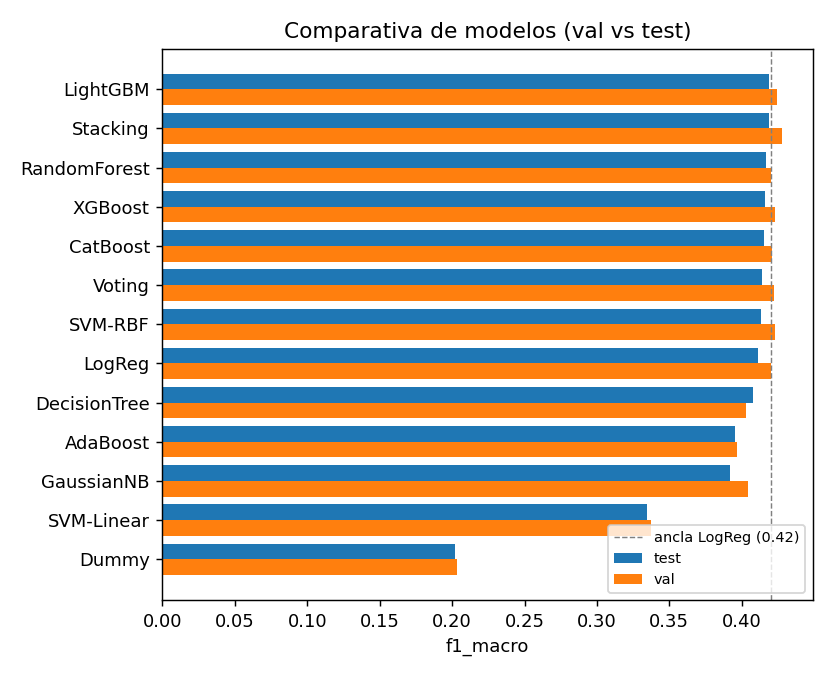
\includegraphics[width=\linewidth]{11_model_comparison.png}
  \end{columns}
\end{frame}

% 17 ----------------------------------------------------------------
\begin{frame}{Visualizaciones del rendimiento}
  \begin{columns}
    \column{0.5\textwidth}
    \centering
    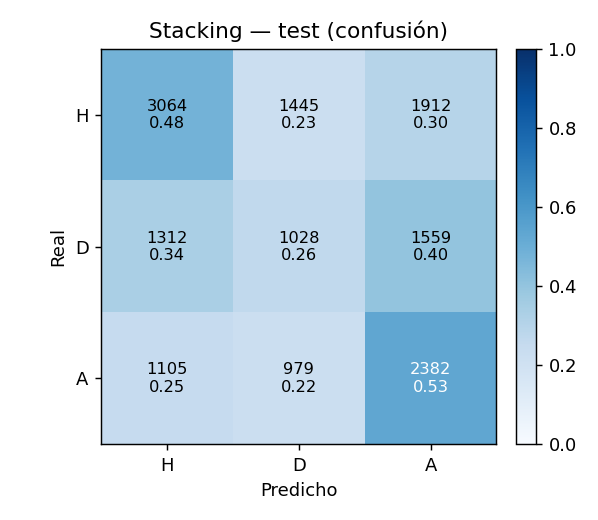
\includegraphics[width=0.85\linewidth]{cm_11_proposed_test.png}\\
    {\footnotesize El empate se lo reparten H y A.}
    \column{0.5\textwidth}
    \centering
    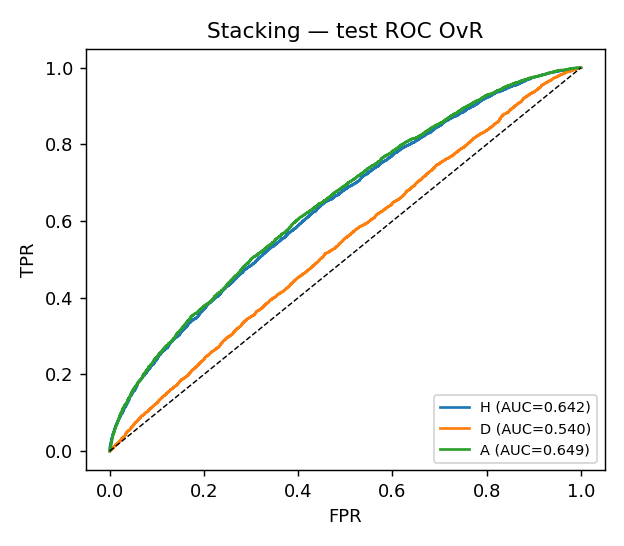
\includegraphics[width=0.9\linewidth]{roc_11_proposed_test.png}\\
    {\footnotesize ROC OvR del modelo propuesto.}
  \end{columns}
\end{frame}

% 18 ----------------------------------------------------------------
\begin{frame}{Análisis estadístico --- Wilcoxon}
  \begin{itemize}
    \item Prueba de rangos con signo ($\alpha=0{,}05$) sobre F1 macro por bloque mensual
    ($n=17$).
    \item Propuesto (Stacking) vs. líneas base:
    \begin{itemize}
      \item vs. Dummy: $p = 7{,}6\times10^{-6}$ \quad\textbf{significativo}
      \item vs. Naive Bayes: $p = 6{,}7\times10^{-4}$ \quad\textbf{significativo}
    \end{itemize}
    \item $\Rightarrow$ la mejora \textbf{no} es producto del azar.
  \end{itemize}
\end{frame}

% 19 ----------------------------------------------------------------
\begin{frame}{Interpretabilidad --- SHAP}
  \begin{columns}
    \column{0.5\textwidth}
    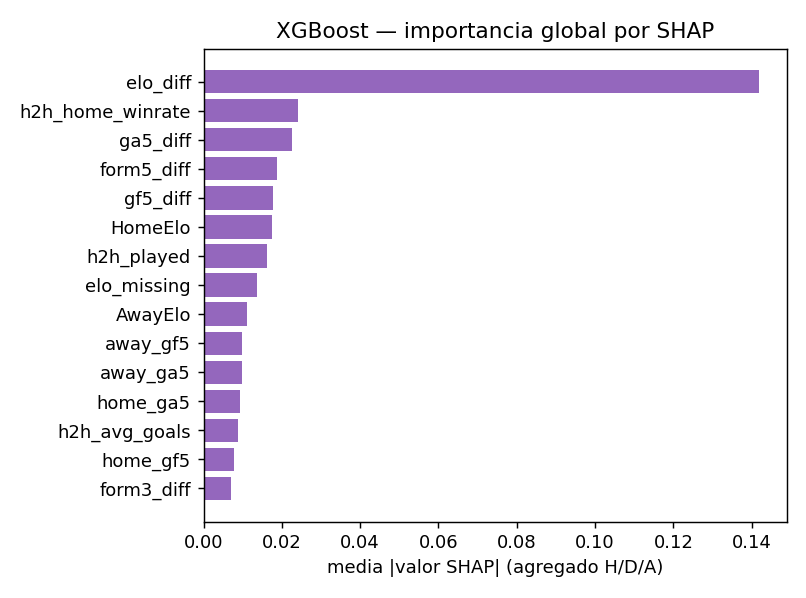
\includegraphics[width=\linewidth]{shap_importance.png}
    \column{0.5\textwidth}
    \begin{itemize}
      \item \textbf{\texttt{elo\_diff}} domina la predicción.
      \item Le siguen historial directo, forma y goles recientes.
      \item Confirmado por importancia de permutación (RF): \emph{dos métodos, misma conclusión}.
    \end{itemize}
  \end{columns}
\end{frame}

% 20 ----------------------------------------------------------------
\begin{frame}{Discusión y amenazas a la validez}
  \begin{itemize}
    \item \textbf{No linealidad:} LinearSVC hunde recall$_D$ a 0,004; SVM-RBF lo sube a 0,31.
    \item \textbf{Desbalance:} \texttt{class\_weight} $>$ SMOTE (el empate no tiene región propia).
    \item \textbf{Validez interna:} sin fuga (no hay accuracies $>65\%$).
    \item \textbf{Validez externa:} sin cuotas $\Rightarrow$ techo inferior; deriva temporal no garantizada.
  \end{itemize}
\end{frame}

% 21 ----------------------------------------------------------------
\begin{frame}{Conclusiones y trabajo futuro}
  \begin{block}{Conclusiones}
    \begin{enumerate}
      \item El empate es un \textbf{límite estructural}, no una falla de los algoritmos.
      \item Frontera no lineal; \texttt{class\_weight} $>$ SMOTE; \texttt{elo\_diff} domina.
      \item El propuesto supera a las bases con \textbf{significancia estadística}.
    \end{enumerate}
  \end{block}
  \begin{block}{Trabajo futuro}
    Incorporar cuotas (medir el salto), calibrar la incertidumbre del empate (RPS),
    modelos secuenciales de la forma.
  \end{block}
\end{frame}

% 22 ----------------------------------------------------------------
\begin{frame}[plain]
  \centering
  \vfill
  {\Large \textbf{Gracias}}\\[1em]
  Repositorio del proyecto y artículo IEEE:\\[0.3em]
  \url{https://github.com/Arbues/football-prediction}\\[1em]
  \emph{¿Preguntas?}
  \vfill
\end{frame}

\end{document}
